\documentclass[11pt,a4paper]{article}
\usepackage[utf8]{inputenc}
\usepackage[T1]{fontenc}
\usepackage{lmodern}
\usepackage{amsmath,amssymb,bm}
\usepackage[margin=2.3cm]{geometry}
\usepackage{booktabs}
\usepackage{xcolor}
\usepackage{graphicx}
\usepackage{tikz}
\usetikzlibrary{arrows.meta,calc,decorations.markings,decorations.pathmorphing,positioning,shapes.geometric,patterns}
\usepackage{pgfplots}
\pgfplotsset{compat=1.18}
\usepackage{circuitikz}
\usepackage[most]{tcolorbox}
\usepackage[colorlinks=true,linkcolor=blue!50!black,citecolor=blue!50!black,urlcolor=blue!50!black]{hyperref}

% ---------------------------------------------------------------- macros
\newcommand{\bB}{\mathbf{B}}
\newcommand{\bJ}{\mathbf{J}}
\newcommand{\bE}{\mathbf{E}}
\newcommand{\bv}{\mathbf{v}}
\newcommand{\bn}{\mathbf{n}}
\newcommand{\bb}{\mathbf{b}}
\newcommand{\ephi}{\mathbf{e}_\varphi}
\newcommand{\eR}{\mathbf{e}_R}
\newcommand{\eZ}{\mathbf{e}_Z}
\newcommand{\gradp}{\nabla_{\!\perp}}
\newcommand{\divg}{\nabla\!\cdot\!}
\newcommand{\Te}{T_e}
\newcommand{\Ti}{T_i}
\newcommand{\cs}{c_s}
\newcommand{\jsat}{j_{\mathrm{sat}}}
\newcommand{\jpar}{j_\parallel}
\newcommand{\Jpar}{J_\parallel}
\newcommand{\jdia}{\mathbf{j}_{\mathrm{dia}}}
\newcommand{\jpol}{\mathbf{j}_{\mathrm{pol}}}
\newcommand{\jvis}{\mathbf{j}_{\mathrm{vis}}}
\newcommand{\pb}[2]{\left[#1,\,#2\right]}
\newcommand{\code}[1]{\texttt{#1}}
\newcommand{\Oh}{\,\Omega}
\newcommand{\tauic}{\tau_{\mathrm{IC}}}
\newcommand{\vE}{\mathbf{v}_E}
\newcommand{\dd}{\mathrm{d}}
\newcommand{\eV}{\,\mathrm{eV}}

\tcbset{
  eli/.style={colback=yellow!8, colframe=orange!70!black, fonttitle=\bfseries, title=#1, breakable},
  key/.style={colback=blue!4, colframe=blue!50!black, fonttitle=\bfseries, title=#1, breakable},
  warn/.style={colback=red!4, colframe=red!60!black, fonttitle=\bfseries, title=#1, breakable},
}

\title{Currents in the scrape-off layer, from scratch\\[4pt]
\large Charge conservation, sheaths, cross-field currents, the three circuits, how SOLPS does it,\\
and what the currents of JOREK's reduced MHD are}
\author{Working notes for the sheath-current paper}
\date{November 2026}

\begin{document}
\maketitle

\begin{abstract}
\noindent
These notes build the physics of scrape-off-layer (SOL) currents from the ground up, with the single goal of being able to
look at a plate-current plot from a divertor simulation and know where every ampere comes from and where it goes.
Part~I introduces the pieces: charge conservation, parallel Ohm's law, the sheath as a nonlinear resistor, and the
currents that cross magnetic field lines. Part~II assembles them into the three circuits found in the literature:
Pfirsch--Schl\"uter, thermoelectric and plate-closing currents, plus the single-plate radial loop that dominates our own
simulation. Part~III shows how SOLPS (B2.5) writes and closes these currents, term by term from its manual and sources.
Part~IV derives, from the perpendicular momentum balance, what currents JOREK's reduced-MHD vorticity equation contains
and how they map onto the SOLPS list, and gives the numbers for the AUG \#33616 case. Part~V reads our results with
these tools. Every equation that matters is derived; every number is traceable.
\end{abstract}

\tableofcontents
\clearpage

% ======================================================================
\section*{How to read these notes}
\addcontentsline{toc}{section}{How to read these notes}

Boxes marked \textbf{ELI5} say the same thing as the surrounding text without equations. Boxes marked \textbf{Key}
are the statements to remember. Boxes marked \textbf{Watch out} are places where it is easy to fool yourself.

\begin{tcolorbox}[key={Sign conventions used throughout}]
\begin{itemize}
\item $j_n > 0$ means \emph{ions} are collected by the wall, i.e.\ conventional current flows from the plasma into
      the wall, at \emph{both} plates. This is the convention of JOREK's \code{Jn\_par} $= -\code{zj}\,B_n/(\mu_0F_0)
      = \bJ_\parallel\cdot\bn$ with the outward normal, and of our plots. Rozhansky et al.\ \cite{rozhansky2020} use the
      \emph{tube} convention instead: positive means current flowing along the field from the inner to the outer
      target, i.e.\ ``to the plate'' at the outer and ``away from the plate'' at the inner target. A plate-to-plate
      (thermoelectric) current has the same sign at both plates in their convention and opposite signs in ours; a plate
      closing current the reverse. Translate before comparing signs.
\item Along a flux tube, $s$ runs from the inner plate ($s=0$) to the outer plate ($s=L$), and a tube current
      $I(s) > 0$ flows from inner to outer. Hence $I(0) = -I_{\mathrm{in}}$ and $I(L) = +I_{\mathrm{out}}$ in terms of
      the plate currents $I_{\mathrm{in}}, I_{\mathrm{out}}$ (ions positive).
\item $\Phi$ is the plasma potential at the sheath entrance, the wall is at $V_w$ (grounded: $V_w = 0$).
\item Temperatures in eV unless $k_B$ is written. $\Lambda \simeq 3$ is the floating sheath drop in units of $\Te/e$.
\end{itemize}
\end{tcolorbox}

% ======================================================================
\part{The pieces}

\section{Charge conservation}

A plasma is quasi-neutral: on scales larger than the Debye length and slower than the plasma frequency, the electron
and ion charge densities are equal to a precision that no transport process can disturb. There is therefore no
charge accumulation anywhere, and the current density obeys
\begin{equation}
  \divg\bJ = 0 \qquad\text{everywhere, at every instant.}
  \label{eq:divj}
\end{equation}
This is the whole content of ``current conservation''. It does not say that current flows along field lines; it says
that whatever flows into a volume flows out of it.

\begin{tcolorbox}[eli={ELI5: water in pipes}]
Think of current as water in a network of pipes that cannot store water. Whatever goes into a junction comes out of it.
A \emph{flux tube} is one pipe with two open ends, the two divertor plates, but its walls are not watertight: water
can also leak through the sides into the neighbouring pipes. The statement ``what goes in at one plate comes out at the
other'' is only true if the walls are watertight. The whole question of this document is how leaky the walls are and
what makes them leak.
\end{tcolorbox}

Integrate \eqref{eq:divj} over the volume of a flux tube bounded by two flux surfaces $\psi_a$, $\psi_b$ and the two
plates (Fig.~\ref{fig:tube}). The divergence theorem gives
\begin{equation}
  \boxed{\;I_{\mathrm{in}} + I_{\mathrm{out}} + I_{\mathrm{sides}} = 0\;}
  \label{eq:tube}
\end{equation}
where $I_{\mathrm{in}}, I_{\mathrm{out}}$ are the currents into the two plates (ions positive) and $I_{\mathrm{sides}}$
is the current leaving through the two flux surfaces. The ``rule'' $I_{\mathrm{in}} = -I_{\mathrm{out}}$ is
\eqref{eq:tube} with $I_{\mathrm{sides}} = 0$. Only currents with a component along $\nabla\psi$ contribute to
$I_{\mathrm{sides}}$. The parallel current never does, since $\bB\cdot\nabla\psi = 0$. So the rule holds exactly if and
only if there is no cross-field current, and the rest of these notes is about the cross-field currents.

\begin{figure}[h]
\centering
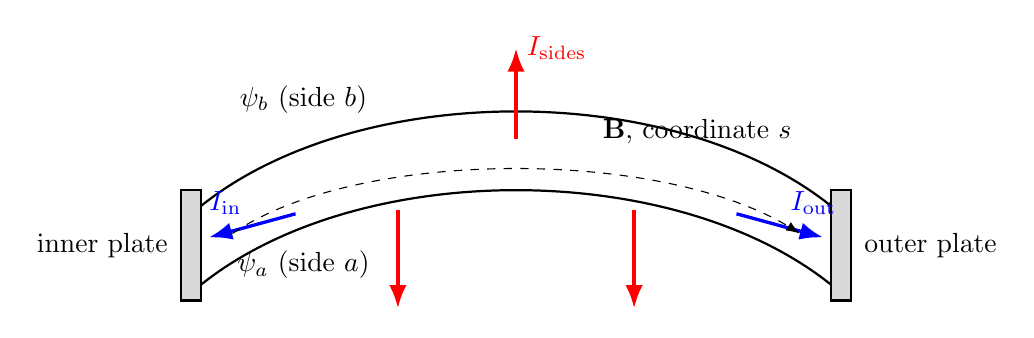
\begin{tikzpicture}[scale=1.0,>=Latex]
  % tube
  \draw[thick] (0,0.0) .. controls (2,1.6) and (6,1.6) .. (8,0.0);
  \draw[thick] (0,-1.0) .. controls (2,0.6) and (6,0.6) .. (8,-1.0);
  \draw[thick,fill=gray!30] (-0.25,-1.2) rectangle (0,0.2);
  \draw[thick,fill=gray!30] (8,-1.2) rectangle (8.25,0.2);
  \node[left] at (-0.3,-0.5) {inner plate};
  \node[right] at (8.3,-0.5) {outer plate};
  \node at (1.3,1.35) {$\psi_b$ (side $b$)};
  \node at (1.3,-0.75) {$\psi_a$ (side $a$)};
  % currents
  \draw[->,very thick,blue] (1.2,-0.1) -- (0.1,-0.4) node[midway,above left] {$I_{\mathrm{in}}$};
  \draw[->,very thick,blue] (6.8,-0.1) -- (7.9,-0.4) node[midway,above right] {$I_{\mathrm{out}}$};
  \draw[->,very thick,red] (4,0.85) -- (4,2.0) node[right] {$I_{\mathrm{sides}}$};
  \draw[->,very thick,red] (2.5,-0.05) -- (2.5,-1.3);
  \draw[->,very thick,red] (5.5,-0.05) -- (5.5,-1.3);
  % field line
  \draw[dashed,->] (0.4,-0.35) .. controls (2,0.75) and (6,0.75) .. (7.6,-0.35);
  \node at (6.3,0.95) {$\bB$, coordinate $s$};
\end{tikzpicture}
\caption{The control volume behind Eq.~\eqref{eq:tube}: a flux tube between two flux surfaces, ending on the two
divertor plates. Blue: plate currents. Red: current through the sides, which only cross-field currents can carry.}
\label{fig:tube}
\end{figure}

\section{Parallel current: Ohm's law along the field}

Electrons are light and move freely along $\bB$. Their parallel momentum balance, neglecting inertia, is the
generalised Ohm's law:
\begin{equation}
  E_\parallel \;=\; \eta_\parallel\,\jpar \;-\; \frac{1}{e n}\,\nabla_\parallel p_e \;-\; \frac{0.71}{e}\,\nabla_\parallel \Te .
  \label{eq:ohm}
\end{equation}
The three terms are: the resistive drop, the electron pressure gradient (electrons pushed along the field by their own
pressure), and the thermal force (electron--ion friction depends on velocity, so a temperature gradient drags
electrons toward the cold end with coefficient $0.71$ for $Z=1$). The parallel Spitzer resistivity is
\begin{equation}
  \eta_\parallel \simeq 5.2\times10^{-5}\,\frac{Z\,\ln\Lambda_c}{\Te[\mathrm{eV}]^{3/2}}\;\Omega\,\mathrm{m},
  \quad
  {\small\begin{array}{l|cccc}
    \Te & 10\eV & 20\eV & 50\eV & 100\eV \\ \hline
    \eta_\parallel\,[\Omega\mathrm{m}] & 2.5\!\times\!10^{-5} & 8.7\!\times\!10^{-6} & 2.2\!\times\!10^{-6} & 7.8\!\times\!10^{-7}
  \end{array}}
  \label{eq:spitzer}
\end{equation}

\paragraph{No current: the Boltzmann relation.}
Put $\jpar = 0$ in \eqref{eq:ohm} and write $E_\parallel = -\nabla_\parallel\Phi$. For isothermal electrons,
\begin{equation}
  \Phi(s) - \Phi(0) = \frac{\Te}{e}\,\ln\frac{n(s)}{n(0)} .
  \label{eq:boltzmann}
\end{equation}
This matters enormously for reading potentials: \emph{two ends of a tube can differ by tens of volts with zero current
flowing}, if their densities and temperatures differ. A potential difference is not a drive for current; only the
departure from \eqref{eq:ohm} with $\jpar=0$ is.

\paragraph{Resistance of a tube.}
For a current $I$ through a tube of cross-section $A(s)$ and length $L$ along the field,
\begin{equation}
  R_{\mathrm{tube}} = \int_0^{L}\frac{\eta_\parallel(s)}{A(s)}\,\dd s .
  \label{eq:rtube}
\end{equation}
For a SOL tube $L \sim 50$--$100\,$m, so even a good conductor is a long wire.

\section{The sheath: a nonlinear resistor at each end}

At a material surface the electrons, being faster, would leave first. The plasma charges positive until the resulting
potential drop in a thin layer (the sheath, a few Debye lengths) repels enough electrons for the two fluxes to balance.
Two standard results \cite{stangeby}:
\begin{align}
  j_{i,n} &= e\,n\,\cs\,|\bb\cdot\bn|, \qquad \cs = \sqrt{\frac{\gamma\,(\Te+\Ti)}{m_i}} &&\text{(Bohm: ions arrive at the sound speed)}
  \label{eq:ji}\\
  j_{e,n} &= e\,n\,\frac{\bar v_e}{4}\,|\bb\cdot\bn|\,\exp\!\Big(-\frac{e(\Phi - V_w)}{\Te}\Big), \qquad
  \bar v_e = \sqrt{\frac{8\Te}{\pi m_e}} &&\text{(Boltzmann-reduced electron flux)}
  \label{eq:je}
\end{align}
The factor $|\bb\cdot\bn|$ projects the parallel flux onto the wall normal; at grazing incidence (2--3$^\circ$ on
divertor targets) it is 0.03--0.05.

\paragraph{Floating potential.} With $j_{i,n} = j_{e,n}$,
\begin{equation}
  \frac{e(\Phi - V_w)}{\Te} = \Lambda \equiv \ln\frac{\bar v_e}{4\cs}
  = \tfrac12\ln\!\Big[\frac{m_i}{2\pi m_e\,\gamma(1+\Ti/\Te)}\Big] \simeq 2.6\text{--}2.8 \text{ (D)},
  \label{eq:lambda}
\end{equation}
and JOREK uses the round constant $\Lambda = 3$. A floating plate point therefore sits at $\Phi \simeq 3\,\Te/e$ above
the wall: 30~V at 10~eV, 165~V at 55~eV.

\paragraph{Current--voltage characteristic.} With a net current, $j_n = j_{i,n} - j_{e,n}$:
\begin{equation}
  \boxed{\;j_n = \jsat\,\big[1 - e^{\,x}\big],\qquad x = \Lambda - \frac{e(\Phi-V_w)}{\Te},\qquad
  \jsat = e\,n\,\cs\,|\bb\cdot\bn| \;}
  \label{eq:char}
\end{equation}
Fig.~\ref{fig:char} shows it. Three regimes: $\Phi$ above floating ($x<0$) collects ions, saturating at $\jsat$;
$\Phi$ at floating carries nothing; $\Phi$ below floating ($x>0$) collects electrons, exponentially, up to electron
saturation at $x = \Lambda$ where $j_n = -(e^\Lambda - 1)\jsat \simeq -19\,\jsat$.

\begin{figure}[h]
\centering
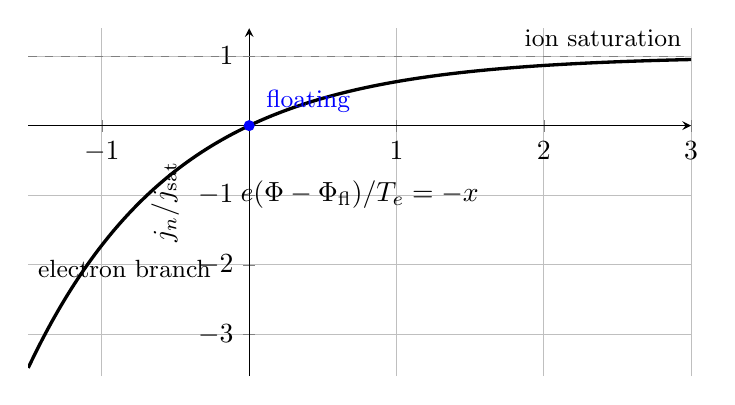
\begin{tikzpicture}
\begin{axis}[width=10cm,height=6cm,xlabel={$e(\Phi-\Phi_{\mathrm{fl}})/\Te = -x$},ylabel={$j_n/\jsat$},
  xmin=-1.5,xmax=3,ymin=-3.6,ymax=1.4,grid=major,axis lines=middle,xlabel near ticks,ylabel near ticks,
  xtick={-1,0,1,2,3},ytick={-3,-2,-1,0,1}]
  \addplot[very thick,black,domain=-1.5:3,samples=200] {1-exp(-x)};
  \addplot[dashed,gray] coordinates {(-1.5,1) (3,1)};
  \node[anchor=south east] at (axis cs:3,1) {\small ion saturation};
  \node[anchor=north west] at (axis cs:-1.5,-1.8) {\small electron branch};
  \node[anchor=south west,blue] at (axis cs:0.05,0.05) {\small floating};
  \fill[blue] (axis cs:0,0) circle (2pt);
\end{axis}
\end{tikzpicture}
\caption{The sheath characteristic, Eq.~\eqref{eq:char}. Ion current is positive. A few $\Te/e$ either side of
floating change the current by order $\jsat$: the sheath is a strongly nonlinear resistor.}
\label{fig:char}
\end{figure}

\paragraph{Small-signal sheath resistance.} Linearising \eqref{eq:char} around floating,
$j_n \simeq -\jsat\,x = \jsat\,(e\,\delta\Phi/\Te)$, so per unit area
\begin{equation}
  R_{\mathrm{sh}} = \frac{\Te}{e\,\jsat}\quad[\Omega\,\mathrm{m^2}],\qquad
  R_{\mathrm{sh}}^{\mathrm{(tube)}} = \frac{\Te}{e\,I_{\mathrm{sat}}}\quad[\Omega] ,
  \label{eq:rsh}
\end{equation}
with $I_{\mathrm{sat}}$ the ion saturation current of the tube's footprint. For a tube that can deliver 1~kA of ion
saturation current at 20~eV, $R_{\mathrm{sh}} = 0.02\,\Omega$. This is the same order as the Spitzer resistance of a
70~m SOL tube, which is why the sheaths cannot be dropped from the thermoelectric circuit.

\begin{tcolorbox}[eli={ELI5: the sheath}]
The plasma in front of a metal wall behaves like a diode with a built-in offset: it sits by itself at about three
times its electron temperature above the wall, in volts. Push it a little higher and ions pour in, up to a limit.
Pull it a little lower and electrons pour in, with no practical limit. Whoever sets the potential in front of the
plate therefore sets the current through it, and the plate, being metal, cannot be at two potentials at once.
\end{tcolorbox}

\section{Currents across the magnetic field}
\label{sec:perp}

Charged particles do not cross field lines freely, but currents across the field exist whenever there is a force on
the fluid perpendicular to $\bB$. Take the ion perpendicular momentum balance, keeping inertia, pressure, viscosity and
friction on neutrals:
\begin{equation}
  \rho\,\frac{\dd\bv_\perp}{\dd t} = \bJ\times\bB - \nabla p + \divg\mathbf{\Pi} - \rho\,\nu_{in}\,(\bv - \bv_n) .
  \label{eq:perpmom}
\end{equation}
Cross with $\bB$ and divide by $B^2$ to solve for the perpendicular current:
\begin{equation}
  \boxed{\;\bJ_\perp = \underbrace{\frac{\bB\times\nabla p}{B^2}}_{\jdia}
  \;+\; \underbrace{\frac{\rho}{B^2}\,\bB\times\frac{\dd\bv_\perp}{\dd t}}_{\jpol}
  \;-\; \underbrace{\frac{\bB\times\divg\mathbf{\Pi}}{B^2}}_{\jvis}
  \;+\; \underbrace{\frac{\rho\nu_{in}}{B^2}\,\bB\times(\bv-\bv_n)}_{\mathbf{j}_{in}}\;}
  \label{eq:jperp}
\end{equation}
Every cross-field current in SOLPS and in JOREK is one of these four, or an ad hoc addition (``anomalous
conductivity''). They are driven by \emph{forces}, not by the electric field directly: the plasma is not an ohmic
conductor across $\bB$. Fig.~\ref{fig:gradb} shows the single-particle origin of the first and most important one.

\begin{figure}[h]
\centering
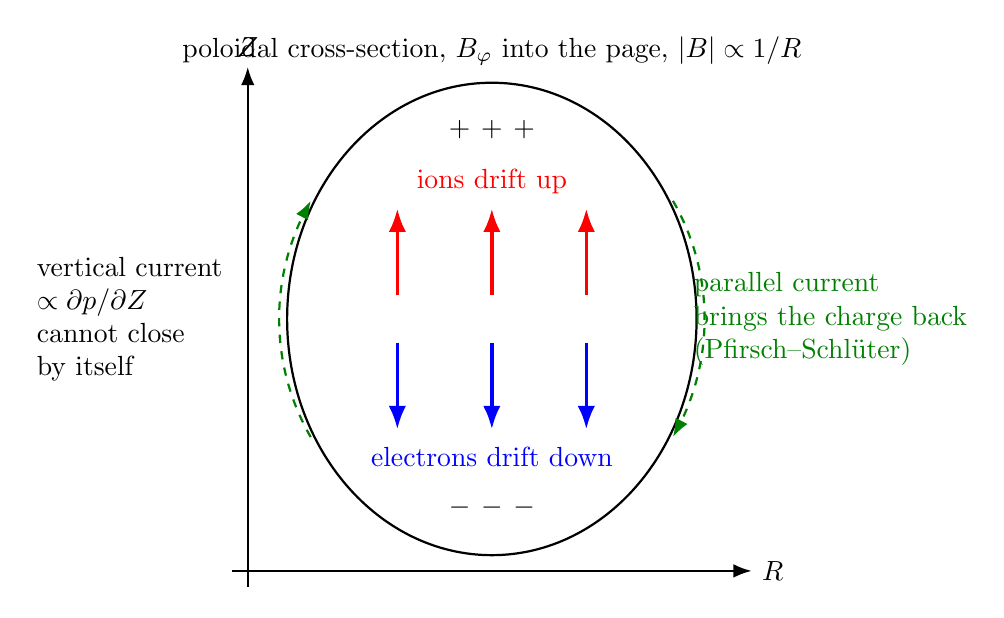
\begin{tikzpicture}[>=Latex,scale=1]
  % torus cross-section: inboard left, outboard right
  \draw[thick] (0,0) ellipse (2.6 and 3.0);
  \node at (0,3.4) {poloidal cross-section, $B_\varphi$ into the page, $|B|\propto 1/R$};
  \draw[->,thick] (-3.3,-3.2) -- (3.3,-3.2) node[right] {$R$};
  \draw[->,thick] (-3.1,-3.4) -- (-3.1,3.2) node[above] {$Z$};
  % grad B drifts
  \foreach \x in {-1.2,0,1.2} {
    \draw[->,red,very thick] (\x,0.3) -- (\x,1.4);
    \draw[->,blue,very thick] (\x,-0.3) -- (\x,-1.4);
  }
  \node[red] at (0,1.75) {ions drift up};
  \node[blue] at (0,-1.75) {electrons drift down};
  \node at (0,2.4) {$+\,+\,+$};
  \node at (0,-2.4) {$-\,-\,-$};
  % return along the field (schematic)
  \draw[->,thick,green!50!black,dashed] (2.3,1.5) arc (30:-30:3.0);
  \draw[->,thick,green!50!black,dashed] (-2.3,-1.5) arc (210:150:3.0);
  \node[green!50!black,align=left] at (4.3,0) {parallel current\\ brings the charge back\\ (Pfirsch--Schl\"uter)};
  \node[align=left] at (-4.6,0) {vertical current\\ $\propto \partial p/\partial Z$\\ cannot close\\ by itself};
\end{tikzpicture}
\caption{The grad-$B$ and curvature drifts separate charges vertically. The resulting vertical current is the
divergence-carrying part of the diamagnetic current. On closed surfaces it is closed by parallel current; on open
field lines that parallel current ends on the plates.}
\label{fig:gradb}
\end{figure}

\subsection{The diamagnetic current and its divergence}
\label{sec:dia}

$\jdia = \bB\times\nabla p/B^2$ is perpendicular to both $\bB$ and $\nabla p$. On a closed surface with $p = p(\psi)$ it
lies inside the flux surface and carries nothing across it. Its divergence, however, is not zero in a torus. Using
$\divg(\mathbf{a}\times\mathbf{c}) = \mathbf{c}\cdot\nabla\times\mathbf{a} - \mathbf{a}\cdot\nabla\times\mathbf{c}$
with $\nabla\times\nabla p = 0$,
\begin{equation}
  \divg\jdia = \nabla p\cdot\nabla\times\Big(\frac{\bB}{B^2}\Big).
\end{equation}
For a tokamak $\bB \simeq (F_0/R)\,\ephi$ to leading order, so $\bB/B^2 \simeq (R/F_0)\,\ephi$, and in cylindrical
coordinates $\nabla\times\big(A_\varphi\ephi\big) = -\partial_Z A_\varphi\,\eR + \tfrac1R\partial_R(R A_\varphi)\,\eZ$
gives $\nabla\times(R\ephi/F_0) = (2/F_0)\,\eZ$ up to the orientation of $\varphi$. Hence
\begin{equation}
  \boxed{\;\divg\jdia = \pm\frac{2}{F_0}\,\frac{\partial p}{\partial Z} = \pm\frac{2}{B R}\,\frac{\partial p}{\partial Z}\;}
  \label{eq:divdia}
\end{equation}
with the upper sign in a right-handed $(R,\varphi,Z)$ basis and the lower sign in JOREK's right-handed $(R,Z,\varphi)$
basis, where $\ephi\times\nabla p = (-\partial_Z p,\,+\partial_R p)$ and $\jdia = (R/F_0)(-\partial_Z p,\,\partial_R p)$,
which is also what the postproc's \code{JR}, \code{JZ} contain.
This is the ``vertical $\nabla B$ current'' of the SOL literature \cite{rozhansky2001,zhao2026}: wherever the pressure
varies vertically, charge is being deposited at the rate \eqref{eq:divdia} and something else must carry it away. On a
closed surface the vertical variation of $p(\psi)$ along the surface is what drives the Pfirsch--Schl\"uter current
(Sec.~\ref{sec:ps}). On open field lines the pressure falls along the divertor legs, which are nearly vertical, so the
legs are strong sources of \eqref{eq:divdia}.

\begin{tcolorbox}[warn={Watch out: ``the diamagnetic current crosses flux surfaces'' is true on open lines}]
With $p = p(\psi)$ the diamagnetic current is tangent to flux surfaces. In the SOL, $p$ also varies \emph{along} the
field line, towards the plates. The poloidal component of that gradient, crossed with the toroidal field, gives a
radial diamagnetic current, $j_{\mathrm{dia},r} \simeq -(B_\varphi/B^2)\,\partial p/\partial s_{\mathrm{pol}}$.
In a flux-tube budget it may enter through one side and leave through the other; its \emph{net} deposit is
\eqref{eq:divdia} integrated over the tube.
\end{tcolorbox}

\subsection{Polarisation current}
The term $\rho\,\dd\bv_\perp/\dd t$ in \eqref{eq:perpmom} with $\bv_\perp \simeq \bE\times\bB/B^2$ gives
\begin{equation}
  \jpol = \frac{\rho}{B^2}\,\frac{\dd\bE_\perp}{\dd t}
        = \frac{\rho}{B^2}\Big(\partial_t + \vE\cdot\nabla\Big)\bE_\perp ,
  \label{eq:jpol}
\end{equation}
the ion inertia responding to a changing perpendicular electric field. It has a time-derivative part, important in
transients (ELMs, a drifting equilibrium) and an advective part, the Reynolds stress of the $E\times B$ flow, which is
present in steady state wherever the flow is sheared. The gyroviscous cancellation adds the diamagnetic velocity to the
advecting flow; the structure stays the same.

\subsection{Viscous current}
A viscous stress $\mathbf{\Pi} = -\mu\nabla\bv$ exerts a force $\mu\nabla^2\bv$; its cross-field current is
$\jvis = -\bB\times\mu\nabla^2\bv_\perp/B^2$. For the $E\times B$ flow, $\bv_E = \bB\times\nabla\Phi/B^2$, so
\begin{equation}
  \divg\jvis \;\simeq\; \frac{\mu}{B^2}\,\nabla_\perp^2\big(\nabla_\perp^2\Phi\big)\cdot\tfrac{1}{B}\cdot B
  \;\propto\; \mu\,\nabla_\perp^2\,\omega,\qquad \omega = \nabla_\perp^2 \Phi/B ,
  \label{eq:jvis}
\end{equation}
a fourth derivative of the potential: viscosity moves charge wherever the vorticity of the $E\times B$ flow is curved.
Shear layers, such as the $E_r$ well at the separatrix, are where this current lives. Its size is set by $\mu$, which
in both SOLPS and JOREK is an anomalous (input) coefficient.

\subsection{Friction and anomalous currents}
Ion--neutral friction gives $\mathbf{j}_{in} \propto \rho\nu_{in}\bB\times\bv/B^2$, important only in cold, neutral-rich
divertors. SOLPS additionally allows an \emph{anomalous perpendicular conductivity},
$\mathbf{j}_{AN} = -\sigma_{AN}\nabla_\perp\Phi$, an ohmic term with no physical derivation, kept as a knob and usually
set small \cite{rozhansky2001}.

\begin{tcolorbox}[key={Key: what carries current across the field}]
Diamagnetic (pressure), polarisation (inertia and Reynolds stress), viscous (shear), ion--neutral friction, and in
SOLPS an optional anomalous ohmic term. None is proportional to the electric field alone. The diamagnetic current is
usually the largest, but on a flux-tube budget it often passes straight through; the \emph{net} cross-field current
into a tube is a competition between its divergence \eqref{eq:divdia} and the inertial and viscous terms.
\end{tcolorbox}

% ======================================================================
\part{The circuits}

\section{Pfirsch--Schl\"uter current on closed surfaces}
\label{sec:ps}

On a closed flux surface with $p=p(r)$, Eq.~\eqref{eq:divj} with \eqref{eq:divdia} requires a parallel current whose
divergence cancels the vertical deposition:
\begin{equation}
  \bB\cdot\nabla\Big(\frac{\jpar}{B}\Big) = -\divg\jdia = -\frac{2}{BR}\,\frac{\partial p}{\partial Z}.
  \label{eq:psode}
\end{equation}
In a large-aspect-ratio circular geometry, $Z = r\sin\theta$, $\partial p/\partial Z = p'(r)\sin\theta$,
$\bB\cdot\nabla = (B_\theta/r)\,\partial_\theta$, $B\simeq B_0$, $R\simeq R_0$:
\begin{equation}
  \frac{B_\theta}{r}\,\partial_\theta\Big(\frac{\jpar}{B_0}\Big) = -\frac{2 p'\sin\theta}{B_0 R_0}
  \quad\Longrightarrow\quad
  \boxed{\;\jpar^{PS} = \frac{2\,q}{B_0}\,p'(r)\,\cos\theta\;},\qquad q = \frac{r B_0}{R_0 B_\theta}.
  \label{eq:ps}
\end{equation}
It is anti-parallel on the outboard side ($p'<0$), parallel on the inboard side, averages to zero over the surface,
and is $q$ times larger than the diamagnetic current it closes. Fig.~\ref{fig:gradb} is the picture. Nothing crosses
the flux surface: the PS current only redistributes charge \emph{within} it. That is why, in a flux-surface average,
the parallel current drops out of charge conservation identically.

\section{Open field lines: currents that end on the plates}

In the SOL, integrating \eqref{eq:psode} along the field from the inner plate gives
\begin{equation}
  \frac{\jpar(s)}{B} = \frac{\jpar(0)}{B} - \int_0^{s}\frac{2}{B^2 R}\,\frac{\partial p}{\partial Z}\,\dd s' .
  \label{eq:psopen}
\end{equation}
Now the current does not have to average to zero: whatever the integral accumulates arrives at the plates. Two things
follow.

\paragraph{The PS current reaches the targets.} Above the X-point the SOL tubes still see $p$ varying along the surface
and the PS pattern of \eqref{eq:ps} forms, but it is now absorbed by the sheaths instead of closing on itself. Schaffer,
Chankin et al.\ measured exactly such current layers at the JET target and found their magnitude and sign fit the SOL
PS current rather than a thermoelectric current \cite{schaffer}.

\paragraph{The legs are sources.} Below the X-point the pressure drops along the near-vertical legs, so
$\partial p/\partial Z$ is large and \eqref{eq:divdia} deposits charge in the legs. Zhao et al.\ write this source as
$\partial\jpar/\partial s \simeq (1/BR)\,\partial p_{\mathrm{tot}}/\partial Z$ and note that the resulting parallel current
``flows away from the location of the strongest source toward both divertor targets'' \cite{zhao2026}. Both targets:
same sign at the two plates. Rozhansky et al.\ call these \emph{plate closing currents of type 1} \cite{rozhansky2020}.

\section{The thermoelectric circuit (Staebler--Hinton)}
\label{sec:thermo}

Now combine Ohm's law \eqref{eq:ohm} along a tube with a sheath at each end \cite{staebler}. Let the tube current be
$I$, positive from inner to outer, so the inner plate collects $-I$ and the outer $+I$ (ions positive). Linearise both
sheaths around floating with \eqref{eq:rsh}:
\begin{equation}
  \Phi_{\mathrm{in}} = \frac{\Te^{\mathrm{in}}}{e}\,\Lambda - R_{\mathrm{sh}}^{\mathrm{in}}\,I,\qquad
  \Phi_{\mathrm{out}} = \frac{\Te^{\mathrm{out}}}{e}\,\Lambda + R_{\mathrm{sh}}^{\mathrm{out}}\,I .
\end{equation}
Integrate \eqref{eq:ohm} from inner to outer with $E_\parallel = -\partial_s\Phi$:
\begin{equation}
  \Phi_{\mathrm{out}} - \Phi_{\mathrm{in}} = -R_{\mathrm{tube}}\,I
  + \int_0^L \frac{\partial_s p_e}{e n}\,\dd s + \frac{0.71}{e}\big(\Te^{\mathrm{out}} - \Te^{\mathrm{in}}\big).
\end{equation}
Eliminate the potentials:
\begin{equation}
  \boxed{\;
  I = -\,\frac{\dfrac{(\Lambda - 0.71)}{e}\,\big(\Te^{\mathrm{out}} - \Te^{\mathrm{in}}\big)
          \;-\; \displaystyle\int_0^L \frac{\partial_s p_e}{e n}\,\dd s}
         {R_{\mathrm{sh}}^{\mathrm{in}} + R_{\mathrm{sh}}^{\mathrm{out}} + R_{\mathrm{tube}}}
  \;}
  \label{eq:thermo}
\end{equation}
Read it as a circuit (Fig.~\ref{fig:circuit}): the open-circuit voltage is the difference of the two floating drops,
$\Lambda\Delta\Te/e$, reduced by the thermal force and by the electron-pressure (Boltzmann) term, driving current
through three resistors in series. With $\Te^{\mathrm{out}} > \Te^{\mathrm{in}}$, $I<0$: in the plasma the current flows
from the hot plate to the cold one, the hot plate collects electrons and the cold plate collects ions. This is the
textbook SOL current, measured on many machines with shunts in the target tiles \cite{kallenbach}.

\begin{figure}[h]
\centering
\begin{circuitikz}[american,scale=1.0]
  \draw (0,0) to[battery1,l_={$\Lambda\Te^{\mathrm{in}}/e$}] (0,2)
        to[R,l={$R_{\mathrm{sh}}^{\mathrm{in}}$}] (2.5,2)
        to[R,l={$R_{\mathrm{tube}}$}] (6,2)
        to[battery1,l_={plasma EMF}] (8,2)
        to[R,l={$R_{\mathrm{sh}}^{\mathrm{out}}$}] (10.5,2)
        to[battery1,l={$\Lambda\Te^{\mathrm{out}}/e$}] (10.5,0) -- (0,0);
  \node at (5.25,-0.4) {grounded plates (metal, $V_w = 0$)};
  \node at (5.25,3.1) {plasma along the flux tube, inner $\to$ outer};
  \draw[->,thick,red] (4,1.4) -- (6.5,1.4) node[midway,below] {$I$};
\end{circuitikz}
\caption{The thermoelectric circuit of Eq.~\eqref{eq:thermo}. Two sheath ``batteries'' with their internal
resistances, the tube resistance $R_{\mathrm{tube}} = \int\eta_\parallel\,\dd s/A$, and the Boltzmann/thermal-force EMF
of the plasma in between, $\int\partial_s p_e/(en) + 0.71\Delta\Te/e$. If the plasma EMF
matches the sheath difference, no current flows even though the two plates sit at very different potentials.}
\label{fig:circuit}
\end{figure}

\begin{tcolorbox}[warn={Watch out: a potential difference between the plates is not a current}]
If both plates float and the Boltzmann term balances $\Lambda\Delta\Te/e$, then $\Phi_{\mathrm{out}} - \Phi_{\mathrm{in}}
= \Lambda\Delta\Te/e$ exactly, tens of volts, with $I = 0$. In our AUG run $\Phi_{\mathrm{out}}-\Phi_{\mathrm{in}}$
equals $\Lambda\Delta\Te/e$ within a few volts on every tube: the circuit is open. The 20--40~V between the plates are
held by the electrons, not dropped across a resistor.
\end{tcolorbox}

\paragraph{Numbers for a SOL tube of AUG.} $\Delta\Te \approx 7$~eV, $L_\parallel \approx 70$~m, footprint delivering
$I_{\mathrm{sat}}\approx 1$~kA at 15--20~eV. Then $R_{\mathrm{sh}} \approx 0.02\,\Omega$ per sheath,
$R_{\mathrm{tube}}^{\mathrm{Spitzer}} \approx 0.02\,\Omega$ for a cross-section of $\sim 0.05\,\mathrm{m^2}$, open-circuit
voltage $\sim 16$~V, so $I_{\mathrm{Spitzer}} \sim 0.3$~kA. With a resistivity 20 times Spitzer,
$R_{\mathrm{tube}} \approx 0.4\,\Omega$ and $I \approx 0.04$~kA. The thermoelectric current is proportional to
$1/\eta_\parallel$ once the tube resistance dominates.

\section{The single-plate radial loop}
\label{sec:loop}

The circuit of Sec.~\ref{sec:thermo} uses two plates. There is a second circuit that needs only one, and it is the one
our sheath-current simulations are dominated by. Along one plate the temperature varies strongly: 55~eV at the strike
point, 12~eV a few centimetres into the SOL. Each flux tube ending there would like to float at its own
$\Lambda\Te/e$: 165~V at the strike point, 36~V on the wing. The plasma cannot sustain a 130~V jump across millimetres
of flux surfaces: the resulting radial electric field is of order $10^5$~V/m, with a sheared $E\times B$ flow whose
polarisation and viscous currents \eqref{eq:jpol}, \eqref{eq:jvis} flow down the potential hill. So $\Phi(\psi)$ settles
at a compromise, and the sheath law \eqref{eq:char} converts the compromise into current (Fig.~\ref{fig:loop}):
\begin{itemize}
\item at the strike point $\Phi < \Lambda\Te/e$: electrons flow into the plate, $j_n < 0$;
\item on the wings $\Phi > \Lambda\Te/e$: ions flow into the plate, $j_n > 0$.
\end{itemize}
Conventional current enters the plasma at the strike point, flows radially outward across the flux surfaces in the
SOL, re-enters the plate on the wings, and returns through the metal. Both plates have a hot spot and wings, so both
show the same sign pattern, and the two plate profiles against $\psi$ have the same sign everywhere, which is the
signature that distinguishes this loop from the thermoelectric one. In the taxonomy of \cite{rozhansky2020} this is a
plate closing current of type~2: a radial current in the SOL above the X-point, closed through the plates. What sets
its magnitude is the cross-field conductance of the shear layer, i.e.\ the viscosity and inertia terms, not the
parallel resistivity.

\begin{figure}[h]
\centering
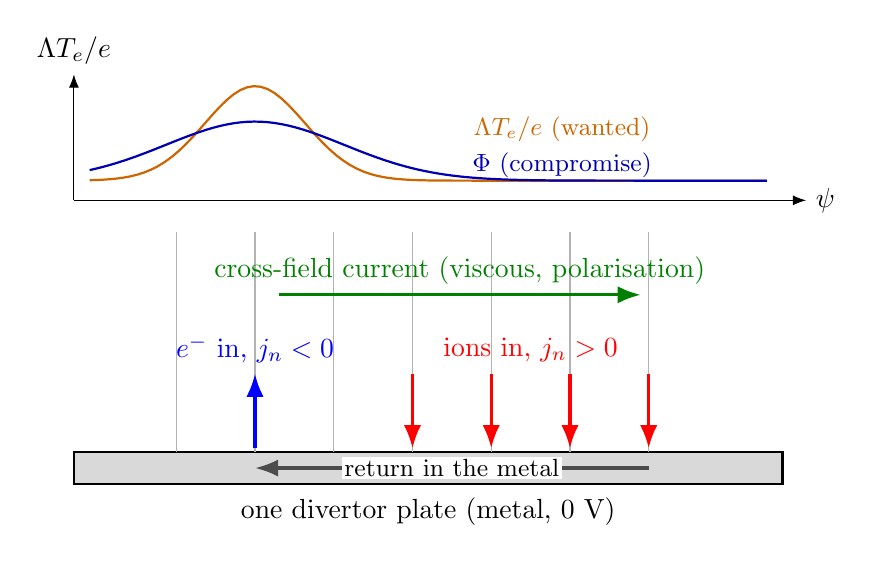
\begin{tikzpicture}[>=Latex,scale=1.0]
  % plate
  \draw[thick,fill=gray!30] (0,0) rectangle (9,-0.4);
  \node at (4.5,-0.75) {one divertor plate (metal, 0 V)};
  % Te profile above
  \begin{scope}[shift={(0,3.2)}]
    \draw[->] (0,0) -- (9.3,0) node[right] {$\psi$};
    \draw[->] (0,0) -- (0,1.6) node[above] {$\Lambda\Te/e$};
    \draw[thick,orange!80!black,domain=0.2:8.8,samples=100] plot (\x,{0.25+1.2*exp(-((\x-2.3)/0.9)^2)});
    \draw[thick,blue!70!black,domain=0.2:8.8,samples=100] plot (\x,{0.25+0.75*exp(-((\x-2.3)/1.6)^2)});
    \node[orange!80!black] at (6.2,0.9) {\small $\Lambda\Te/e$ (wanted)};
    \node[blue!70!black] at (6.2,0.45) {\small $\Phi$ (compromise)};
  \end{scope}
  % flux surfaces (vertical lines)
  \foreach \x in {1.3,2.3,3.3,4.3,5.3,6.3,7.3} \draw[gray!60] (\x,0) -- (\x,2.8);
  % currents at the plate
  \draw[->,very thick,blue] (2.3,0.05) -- (2.3,1.0) node[above] {$e^-$ in, $j_n<0$};
  \foreach \x in {4.3,5.3,6.3,7.3} \draw[->,very thick,red] (\x,1.0) -- (\x,0.05);
  \node[red] at (5.8,1.3) {ions in, $j_n>0$};
  % radial current in the plasma
  \draw[->,very thick,green!50!black] (2.6,2.0) -- (7.2,2.0) node[midway,above] {cross-field current (viscous, polarisation)};
  % return in the metal
  \draw[->,very thick,black!70] (7.3,-0.2) -- (2.3,-0.2);
  \node at (4.8,-0.2) [fill=white,inner sep=1pt] {\small return in the metal};
\end{tikzpicture}
\caption{The single-plate radial loop. The plate is one conductor; the plasma in front of it wants a different floating
potential on every flux surface. Cross-field currents smooth $\Phi(\psi)$, the sheath law turns the mismatch into
electron collection at the hot spot and ion collection on the wings, and the metal closes the loop.}
\label{fig:loop}
\end{figure}

\section{Putting the families together}

Rozhansky et al.\ \cite{rozhansky2020}, from SOLPS-ITER simulations of ASDEX Upgrade and Globus-M, state that the
measured plate currents are the sum of three families (Table~\ref{tab:families}). The single-plate loop of
Sec.~\ref{sec:loop} is their type~2 plate closing current viewed from the plate. Fig.~\ref{fig:families} sketches where
each flows.

\begin{table}[h]
\centering
\begin{tabular}{p{3.2cm}p{4.6cm}p{3.4cm}p{3.4cm}}
\toprule
family & drive & path & sign at the two plates \\
\midrule
Pfirsch--Schl\"uter & $\partial p/\partial Z$ on a surface above the X-point & along the surface; on open lines ends on the plates & opposite (it is a parallel current pattern) \\
thermoelectric & $\Lambda\Delta\Te$ between the plates minus the plasma EMF & along the tube, plate to plate & opposite: hot plate electrons, cold plate ions \\
plate closing, type 1 & vertical $\nabla B$ current of the legs, Eq.~\eqref{eq:divdia} & leg $\to$ both plates & same \\
plate closing, type 2 & radial currents in the SOL above the X-point (viscous, inertial, anomalous) & SOL $\to$ both plates & same \\
\bottomrule
\end{tabular}
\caption{The current families of the SOL after \cite{rozhansky2020,sorokina}. In the SOL the type-1 PCC adds to the
thermoelectric current, in the private region it subtracts from it.}
\label{tab:families}
\end{table}

\begin{figure}[h]
\centering
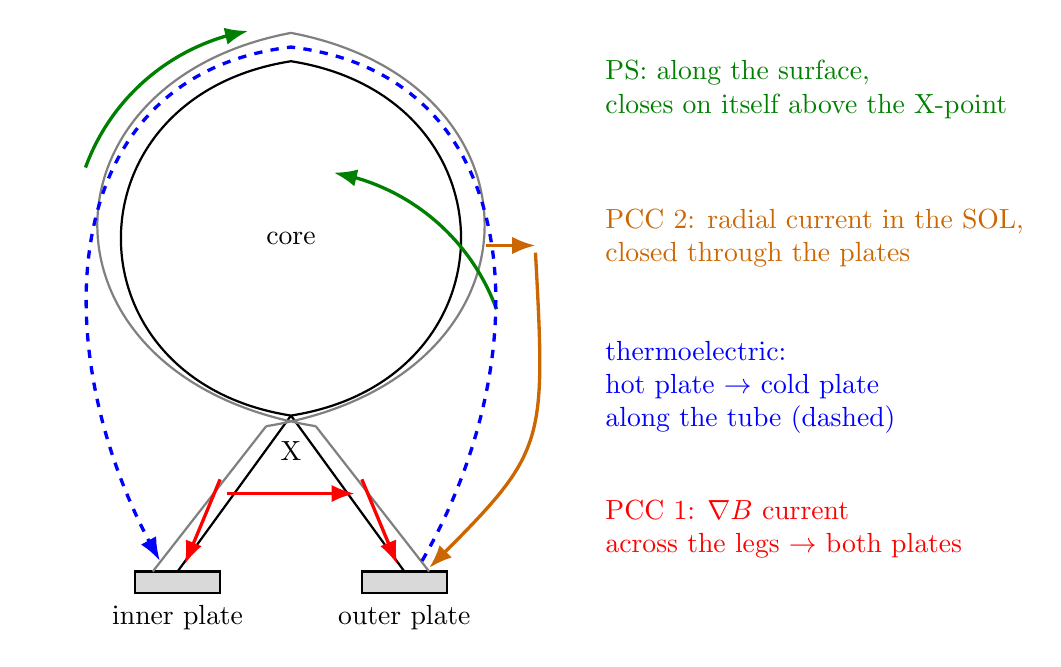
\begin{tikzpicture}[>=Latex,scale=0.9]
  % separatrix-like shape with X-point and legs
  \draw[thick] (0,0) .. controls (-3.2,0.5) and (-3.2,4.5) .. (0,5) .. controls (3.2,4.5) and (3.2,0.5) .. (0,0);
  \draw[thick] (0,0) -- (-1.6,-2.2);
  \draw[thick] (0,0) -- (1.6,-2.2);
  \draw[thick,fill=gray!30] (-2.2,-2.2) rectangle (-1.0,-2.5);
  \draw[thick,fill=gray!30] (1.0,-2.2) rectangle (2.2,-2.5);
  \node at (-1.6,-2.85) {inner plate};
  \node at (1.6,-2.85) {outer plate};
  % SOL surface
  \draw[thick,gray] (0.35,-0.15) .. controls (-3.7,0.5) and (-3.7,4.7) .. (0,5.4) .. controls (3.7,4.7) and (3.7,0.5) .. (-0.35,-0.15);
  \draw[thick,gray] (0.35,-0.15) -- (1.95,-2.2);
  \draw[thick,gray] (-0.35,-0.15) -- (-1.95,-2.2);
  \node at (0,2.5) {core};
  \node at (0,-0.5) {X};
  % PS (green) along SOL surface above X-point
  \draw[->,very thick,green!50!black] (2.9,1.5) arc (20:80:3.0);
  \draw[->,very thick,green!50!black] (-2.9,3.5) arc (160:100:3.0);
  \node[green!50!black,align=left,anchor=west] at (4.3,4.6) {PS: along the surface,\\ closes on itself above the X-point};
  % thermoelectric (blue) plate to plate along the SOL tube
  \draw[->,very thick,blue,dashed] (1.85,-2.05) .. controls (3.5,0.8) and (3.4,4.8) .. (0,5.2) .. controls (-3.4,4.8) and (-3.5,0.8) .. (-1.85,-2.05);
  \node[blue,align=left,anchor=west] at (4.3,0.4) {thermoelectric:\\ hot plate $\to$ cold plate\\ along the tube (dashed)};
  % PCC type 1: vertical in the legs to both plates
  \draw[->,very thick,red] (-1.0,-0.9) -- (-1.5,-2.1);
  \draw[->,very thick,red] (1.0,-0.9) -- (1.5,-2.1);
  \draw[->,very thick,red] (-0.9,-1.1) -- (0.9,-1.1);
  \node[red,align=left,anchor=west] at (4.3,-1.6) {PCC 1: $\nabla B$ current\\ across the legs $\to$ both plates};
  % PCC type 2: radial in the SOL above X-point, then down to plates
  \draw[->,very thick,orange!80!black] (2.75,2.4) -- (3.45,2.4);
  \draw[->,very thick,orange!80!black] (3.45,2.3) .. controls (3.6,-0.5) .. (1.95,-2.15);
  \node[orange!80!black,align=left,anchor=west] at (4.3,2.5) {PCC 2: radial current in the SOL,\\ closed through the plates};
\end{tikzpicture}
\caption{Where the families flow, schematically. Green: Pfirsch--Schl\"uter pattern. Blue: thermoelectric current
from the hotter to the colder plate. Red: plate closing current of type~1, the vertical $\nabla B$ current of the legs
returning through both plates. Orange: type~2, a radial SOL current above the X-point returning through the plates.}
\label{fig:families}
\end{figure}

\paragraph{What the per-tube sum measures.} Returning to \eqref{eq:tube}: the thermoelectric and PS parts have opposite
signs at the two ends and cancel in $I_{\mathrm{in}} + I_{\mathrm{out}}$; the plate closing parts have the same sign and
add. So
\begin{equation}
\begin{aligned}
  \tfrac12\,(I_{\mathrm{out}} - I_{\mathrm{in}}) &= \text{current through the tube (thermoelectric + PS reaching the plates)},\\
  I_{\mathrm{in}} + I_{\mathrm{out}} &= \text{plate closing current} = -I_{\mathrm{sides}} .
\end{aligned}
\label{eq:decomp}
\end{equation}
The colleague's rule says the second is zero. In a code with cross-field currents it is a measurement of them.

\section{What experiments see}

\begin{itemize}
\item \textbf{Thermoelectric currents} are routinely measured with shunts in the divertor tiles. On ASDEX Upgrade they
      flow from the hotter outer to the colder inner target in attached L- and H-mode and reverse when the outer target
      detaches first; they are large enough to matter for the power balance \cite{kallenbach}.
\item \textbf{Pfirsch--Schl\"uter layers} were identified at the JET target by Schaffer, Chankin et al.: narrow current
      layers whose sign and size fit the SOL PS current, passing through the recycling zone and the sheath
      \cite{schaffer}.
\item \textbf{ELM currents}: on TCV, Pitts et al.\ measured target currents during ELMs comparable to the ion saturation
      current, with current, floating potential and $\Te$ arriving in that order \cite{pitts}.
\item \textbf{Detachment}: SOLPS-ITER work by Senichenkov et al.\ finds that when both divertors detach the thermal
      current collapses and the net plate current drops to the size of the radial current leaving through the outer SOL
      and private-flux boundaries of the simulation domain \cite{senichenkov}.
\item \textbf{Closing versus thermoelectric}: in UEDGE simulations of DIII-D detachment, Zhao et al.\ estimate the
      thermoelectric current an order of magnitude below the parallel closing current of the $\nabla B$ source
      \cite{zhao2026}.
\end{itemize}

% ======================================================================
\part{How SOLPS does it}

\section{The B2.5 current equation}

SOLPS (B2.5) solves the current continuity equation \eqref{eq:divj} for the electrostatic potential on its
$(x,y)$ grid, $x$ along and $y$ across the flux surfaces (manual eq.~B.13 / C.191):
\begin{equation}
  \frac{1}{\sqrt g}\,\frac{\partial}{\partial x}\Big(\frac{\sqrt g}{h_x}\,\tilde j_x\Big)
  + \frac{1}{\sqrt g}\,\frac{\partial}{\partial y}\Big(\frac{\sqrt g}{h_y}\,\tilde j_y\Big) = 0,
  \qquad \tilde j_x = b_z\,\tilde j_\perp + b_x\,\jpar .
  \label{eq:solpscc}
\end{equation}
The tilde means ``effective'': divergence-free parts of the diamagnetic current are removed analytically because they
cannot be represented stably on the grid, keeping only the part with the same divergence \cite{rozhansky2001}. The
radial current (manual C.211--C.229) is the sum
\begin{equation}
  j_y = j^{(AN)}_y + \tilde j^{(dia)}_y + j^{(in)}_y + \tilde j^{(vis\parallel)}_y + j^{(vis\perp)}_y
      + \tilde j^{(visq)}_y + \tilde j^{(s)}_y + j^{(ST)}_y ,
  \label{eq:solpsjy}
\end{equation}
with, for a single main ion species,
\begin{align}
  j^{(AN)}_y &= -\sigma^{(AN)}\,\frac{\partial\Phi}{h_y\partial y},
  && \sigma^{(AN)} = \big(c_{\sigma,0} + c_{\sigma,1}\tfrac{10^{20}}{n_e} + \dots\big)\,e\,n_e,\ c_{\sigma,0}\sim10^{-6}\text{--}10^{-3}
  \label{eq:solpsan}\\
  \tilde j^{(dia)}_y &= -B_z\,n\,(\Te+\Ti)\,\frac{\partial}{h_x\partial x}\Big(\frac{1}{B^2}\Big),
  && \text{(vertical $\nabla B$ current, cf.\ \eqref{eq:divdia})}
  \label{eq:solpsdia}\\
  j^{(in)}_y &= -\frac{B_z}{2}\,\frac{\partial}{h_x\partial x}\Big(\frac{1}{B^2}\Big)\,m\,n\,V_\parallel^2,
  && \text{(inertia of the parallel flow)}
  \label{eq:solpsin}\\
  j^{(vis\perp)}_y &= -\frac{1}{B\sqrt g}\,\frac{\partial}{\partial y}\Big(\frac{\sqrt g}{h_y}\,\frac{\eta^{(AN)}}{4}\,\frac{\partial \tilde V_\perp}{h_y\partial y}\Big),
  && V_\perp = -\frac{1}{B h_y}\frac{\partial\Phi}{\partial y} - \frac{1}{e n B h_y}\frac{\partial n\Ti}{\partial y}
  \label{eq:solpsvis}\\
  \tilde j^{(s)}_y &= -\sigma_{in}\Big(\frac{\partial\Phi}{h_y\partial y} + \frac{1}{en}\frac{\partial n\Ti}{h_y\partial y} + B V_{n\perp}\Big),
  && \sigma_{in} = \frac{\tilde\mu\, m_p\, n\, n_n\langle V\sigma_{cx}\rangle}{B^2}
  \label{eq:solpsin2}
\end{align}
plus the parallel-viscosity and heat-viscosity currents (small corrections, needed on closed surfaces to make the
surface-averaged radial current vanish) and an optional stochastic-layer conductivity. Term by term this is
Eq.~\eqref{eq:jperp}: \eqref{eq:solpsdia} is the diamagnetic current written through $\partial(1/B^2)$, which with
$B\propto1/R$ is the same $\partial p/\partial Z$ source as \eqref{eq:divdia}; \eqref{eq:solpsin} is the inertial term;
\eqref{eq:solpsvis} the perpendicular viscous current acting on the $E\times B$ plus diamagnetic flow, with an anomalous
viscosity $\eta^{(AN)} = m n D^{(AN)}$; \eqref{eq:solpsin2} the ion--neutral friction; \eqref{eq:solpsan} the anomalous
conductivity. The parallel current is algebraic, from Ohm's law \eqref{eq:ohm} with Spitzer (or Zhdanov) conductivity;
there is no induction equation.

\section{Boundary conditions for the potential}

The potential equation needs a current condition on every boundary (manual C.7.3 and the routine \code{b2stbc\_phys.F}).

\paragraph{Targets (west/east).} \code{BCPOT = 3} or \code{11} impose the sheath characteristic as the current flux
through the target face,
\begin{equation}
  \frac{\sqrt g}{h_x}\,j_x\Big|_{W} = \frac{\sqrt g}{h_x}\,e\Big[\sum_a z_a\Gamma_{ax}
  + (1-\gamma_e)\,|b_x|\,n_e\,\frac{1}{\sqrt{2\pi}}\sqrt{\frac{\Te}{m_e}}\,
  \exp\!\Big(-\frac{e(\Phi - p_{\Phi,2})}{\Te}\Big)\Big]_W ,
  \label{eq:bcpot}
\end{equation}
i.e.\ ion flux minus Boltzmann-reduced electron flux: exactly \eqref{eq:char} in flux form, linearised in $\Phi$ in the
guard cell. \code{BCPOT = 11} is the version consistent with the drift-compatible Bohm conditions
(\code{BCCON = 14}, \code{BCMOM = 13}, \code{BCENE = 15}).

\paragraph{Radial boundaries (north = outer SOL edge, south = core and private-flux floor).} There is no sheath. The
options are: prescribed potential (1), prescribed gradient (2), prescribed current density (5) or total current
(6, 8, 10 with feedback), decay length (9), and the options 12 and 13 that add the diamagnetic, inertial and other
perpendicular currents of the adjacent cell to the boundary flux, so that the physical cross-field current is allowed
to leave; which of these contributions are included is governed by \code{b2stbc\_istyle\_cur\_contr\_on\_S\_and\_N}
(default 2). At the core boundary the usual choice is zero net current.

\begin{tcolorbox}[key={Key: why SOLPS budgets always close}]
Every current in \eqref{eq:solpsjy} and every boundary condition is a face flux of a finite-volume cell, and the plate
current is itself the face flux \eqref{eq:bcpot}. The sum of all boundary currents is therefore zero to round-off,
\emph{and each boundary's share is a printed number}. Per flux tube, however, $I_{\mathrm{in}} + I_{\mathrm{out}} \neq 0$
whenever \eqref{eq:solpsjy} is non-zero on the tube's sides, which is the normal case near the separatrix.
\end{tcolorbox}

\section{What SOLPS results look like}

Rozhansky's 2001 paper established that the potential near the separatrix is set by the effective perpendicular
conductivity, mostly the diamagnetic current balanced by parallel viscosity, inertia and ion-neutral friction, while
far out in the SOL it is set by the electron parallel force balance, i.e.\ Boltzmann and the sheaths, and is a weak
function of the cross-field conductivity \cite{rozhansky2001}. Target-current comparisons with ASDEX Upgrade probes
only fit when all drifts, and with them all closing currents, are switched on \cite{coster}. In single-null attached
AUG plasmas the thermoelectric current usually dominates the plate totals, with the plate closing currents as the
second component; in connected double-null the thermoelectric drive is weak and the plate closing currents take over
\cite{rozhansky2020}. In double detachment the thermal current collapses and the plate totals shrink to the radial
boundary currents \cite{senichenkov}.

% ======================================================================
\part{The currents of JOREK's reduced MHD}

\section{Fields, variables and units}

Model600 (and the other reduced-MHD models) represents the magnetic field and the velocity as
\begin{equation}
  \bB = F_0\nabla\varphi + \nabla\psi\times\nabla\varphi,\qquad
  \bv = \vE + V_\parallel\bB + \bv_{\mathrm{dia}},\qquad
  \vE = -R\,\nabla u\times\ephi,\qquad \Phi = F_0\,u ,
  \label{eq:jorekfields}
\end{equation}
with $F_0 = R B_\varphi$ constant, $\psi$ the poloidal flux per radian, and $u$ the stream function of the
$E\times B$ flow. The toroidal current is carried by the variable $j$:
\begin{equation}
  j \equiv \Delta^*\psi = R\,\divg\Big(\frac{\nabla\psi}{R}\Big) = -\mu_0 R\,J_\varphi ,
  \qquad
  \Jpar = J_\varphi\,\frac{R|B|}{F_0}\;\Rightarrow\; \frac{\Jpar}{|B|} = -\frac{j}{\mu_0 F_0} .
  \label{eq:jorekj}
\end{equation}
Normalisation: lengths in metres, $\bB$ in tesla, $\rho_0 = m_i n_0$ with $n_0 = 10^{20}\,\mathrm{m^{-3}}\times$
\code{central\_density}; time in units of $t_0 = \sqrt{\mu_0\rho_0}$, velocities in $1/t_0$, pressure $p_{SI} = p/\mu_0$,
current $\bJ_{SI} = \bJ/\mu_0$, potential $\Phi_{SI} = \Phi/t_0$. For AUG \#33616 ($n_0 = 0.765\times10^{20}$,
deuterium): $t_0 = 5.67\times10^{-7}$~s, one normalised unit of $\Phi$ is $1.76\times10^{6}$~V.

Two facts shape everything below. First, $\Jpar$ is \emph{not algebraic}: $\psi$ obeys an induction equation, so the
parallel current is a dynamical variable with its own time scale. Second, the perpendicular currents are \emph{never
stored}: there is no variable for $\bJ_\perp$. They exist only through their divergence, in the equation that
determines $u$.

\section{Ohm's law in JOREK: the induction equation}

The $\psi$ row of model600, in the weak form the code assembles \cite{ohmnote}, is
\begin{equation}
\begin{aligned}
  \frac{1}{R}\,\partial_t\psi = {}& \frac{\eta(\Te)}{R}\,(j - j_s - j_b)
  + \Big(\pb{\psi}{u} - \frac{F_0}{R}\partial_\varphi u\Big)
  - \divg\big(\eta_{\mathrm{num}}\nabla j\big) \\
  & - \frac{2\tauic F_0^2}{\rho_c B^2 R^2}\Big(\pb{\psi}{p_e} - \frac{F_0}{R}\partial_\varphi p_e\Big)
  - \frac{2\tauic\,c\,F_0^2}{B^2R^2}\Big(\pb{\psi}{\Te} - \frac{F_0}{R}\partial_\varphi\Te\Big),
\end{aligned}
\label{eq:jorekohm}
\end{equation}
with the bracket $\pb{a}{b} = \partial_R a\,\partial_Z b - \partial_Z a\,\partial_R b$, the identity
$\pb{\psi}{f} - (F_0/R)\partial_\varphi f = -R\,\bB\cdot\nabla f$, and $2\tauic = 1/(e F_0\sqrt{\mu_0\rho_0})$ the
normalised $1/(en)$ coefficient. Reading the terms with $E_\parallel$ in mind: resistive drop ($\eta$, with the
\code{keep\_current\_prof} source $j_s$ and bootstrap $j_b$ subtracted), the $E\times B$ advection of flux (the
$-\nabla\Phi$ part of $E_\parallel$), hyper-resistivity (numerical), electron pressure gradient and thermal force with
$c = 0.71$ (\code{thermoelectric\_ohm}). This is \eqref{eq:ohm} projected on the toroidal direction and integrated in
time. The resistivity is
\begin{equation}
  \eta(T) = \eta_0\,\Big(\frac{T}{T_0}\Big)^{-3/2}\quad(\code{eta\_T\_dependent}),\qquad
  \eta_{SI} = \mu_0\,\frac{\eta_0}{t_0}\Big(\frac{T}{T_0}\Big)^{-3/2},
  \label{eq:joreketa}
\end{equation}
with $T_0$ the axis temperature of the initial profile.

\section{Deriving the currents of the vorticity equation}
\label{sec:vort}

The $u$ row of model600 (\code{rhs\_ij(var\_u)}) is, in strong form \cite{ernote},
\begin{equation}
\begin{aligned}
  R\,\divg\big(R^2\rho\,\gradp\partial_t u\big)
  &= \underbrace{\tfrac12\pb{R^2|\gradp u|^2}{R^2\rho} + \pb{R^4\rho\,\omega}{u}}_{\text{(a) inertia, Reynolds stress}}
   + \underbrace{\pb{\psi}{j} - \frac{F_0}{R}\,\partial_\varphi j}_{\text{(b) parallel current}}
   - \underbrace{\pb{R^2}{p}}_{\text{(c) diamagnetic}} \\
  &\quad + \underbrace{R\,\mu\,\nabla^2_{\mathrm{pol}}\omega + \mathcal{V}_{\mathrm{num}}}_{\text{(d) viscosity, hyperviscosity}}
   + \underbrace{\mathcal{G}[\tauic,p_i,u]}_{\text{(e) gyroviscous}}
   + \mathcal{N}_{\mathrm{neo}} + \mathcal{S}_u ,
   \qquad \omega = \nabla^2_{\mathrm{pol}}u .
\end{aligned}
\label{eq:vort}
\end{equation}
We now show that this is $F_0 R\,\divg\bJ = 0$ with $\bJ$ the currents of Sec.~\ref{sec:perp}, evaluated with the
reduced-MHD field $\bB\simeq(F_0/R)\ephi$, so that $\bB/B^2 \simeq (R/F_0)\ephi$. JOREK's basis $(R,Z,\varphi)$ is
right-handed: $\eR\times\eZ = \ephi$, $\ephi\times\eR = \eZ$, $\ephi\times\eZ = -\eR$, hence for a poloidal gradient
$\ephi\times\nabla f = (-\partial_Z f,\,+\partial_R f)$ in $(R,Z)$ components. (With this orientation
$B_R = \partial_Z\psi/R$, $B_Z = -\partial_R\psi/R$ and $\pb{\psi}{f} = -R\,\bB_{\mathrm{pol}}\!\cdot\!\nabla f$, as in
the code.)

\paragraph{(c) The diamagnetic current.}
$\jdia = \bB\times\nabla p/B^2 = (R/F_0)\,\ephi\times\nabla p = (R/F_0)\,(-\partial_Z p,\,\partial_R p)$. Its divergence,
\begin{equation}
  \divg\jdia = -\frac{1}{R}\partial_R\Big(\frac{R^2}{F_0}\partial_Z p\Big) + \partial_Z\Big(\frac{R}{F_0}\partial_R p\Big)
  = -\frac{2}{F_0}\,\partial_Z p
  \quad\Longrightarrow\quad
  F_0 R\,\divg\jdia = -2R\,\partial_Z p = -\pb{R^2}{p}.
  \label{eq:cterm}
\end{equation}
This is term (c) exactly: the code assembles it as $+R^2\pb{v}{p}$ against the test function $v$
(\code{factor(var\_u,4)}), whose strong form after integration by parts is $-\pb{R^2}{p}$. It is \eqref{eq:divdia}:
the curvature term of the reduced-MHD vorticity equation is the vertical $\nabla B$ current source of the SOL
literature. JOREK contains the drive of the Pfirsch--Schl\"uter current
and of the type-1 plate closing current.

\paragraph{(b) The parallel current.}
$\divg(\Jpar\bb) = \bB\cdot\nabla(\Jpar/B)$ and, from \eqref{eq:jorekj} in normalised units ($\mu_0 = 1$),
$\Jpar/B = -j/F_0$. With $\bB\cdot\nabla f = -\tfrac1R\big(\pb{\psi}{f} - \tfrac{F_0}{R}\partial_\varphi f\big)$,
\begin{equation}
  F_0 R\,\divg(\Jpar\bb) = F_0 R\,\Big(-\frac{1}{F_0}\Big)\Big(-\frac1R\Big)\Big(\pb{\psi}{j} - \frac{F_0}{R}\partial_\varphi j\Big)
  = \pb{\psi}{j} - \frac{F_0}{R}\,\partial_\varphi j ,
  \label{eq:bterm}
\end{equation}
term (b). In an axisymmetric state the $\partial_\varphi$ part vanishes and $\pb{\psi}{j}$ is $-R\,\bB_{\mathrm{pol}}\cdot\nabla j$:
the variation of the parallel current along the poloidal projection of the field line.

\paragraph{(lhs) and (a) The polarisation current.}
With $\vE = -R\nabla u\times\ephi$ and $\bB/B^2\simeq(R/F_0)\ephi$,
$\bB\times\rho\,\partial_t\vE/B^2 = \rho\,(R/F_0)\,\ephi\times\big(-R\,\partial_t\nabla u\times\ephi\big)
= -(\rho R^2/F_0)\,\gradp\partial_t u$, using $\ephi\times(\mathbf{a}\times\ephi) = \mathbf{a}$ for poloidal $\mathbf{a}$. So
\begin{equation}
  F_0 R\,\divg\jpol^{(\partial_t)} = -R\,\divg\big(\rho R^2\gradp\partial_t u\big),
  \label{eq:lhsterm}
\end{equation}
which is minus the left-hand side of \eqref{eq:vort}: moving it across gives the equation as written. The advective
part $\rho\,(\vE\cdot\nabla)\vE$ produces, after the same manipulation and an integration by parts, the two brackets of
term (a): the Reynolds stress of the $E\times B$ flow, $\pb{R^4\rho\omega}{u}$, and the kinetic-energy bracket. The
gyroviscous block (e) corrects the advecting velocity from $\vE$ to $\vE + \bv_{\mathrm{dia}}$ (the gyroviscous
cancellation), as in B2.5 where inertia and gyroviscosity are combined for the same reason.

\paragraph{(d) The viscous current.}
Physically $\jvis = -\bB\times\mu\nabla^2\vE/B^2 \simeq (\mu R^2/F_0)\,\gradp\omega$ with $\omega = \nabla^2_{\mathrm{pol}}u$.
The code has two forms (\code{visco\_old\_setup}). The old one, used in the AUG case, assembles
$-\mu R\,\nabla v\!\cdot\!\nabla\omega$, i.e.\ $F_0R\,\divg\jvis = \divg(\mu R\nabla\omega)$ and
$\jvis = (\mu/F_0)\gradp\omega$: the $R^2$ of the physical form is absorbed into the definition of $\mu$. The new one
assembles $-\mu R^3\nabla v\!\cdot\!\nabla\omega - 2\mu R^2\omega\,\partial_R v$, i.e.\
$F_0R\,\divg\jvis = \divg(\mu R^3\nabla\omega) + \partial_R(2\mu R^2\omega)$, the physical form. The hyperviscosity
$-\mu_{\mathrm{num}}\,\nabla^2 v\,\nabla^2\omega$ is a numerical current of the same family.

\begin{tcolorbox}[key={Key: the currents JOREK has}]
The vorticity equation \eqref{eq:vort} is $F_0 R\,\divg\bJ = 0$ with
\begin{align*}
  \bJ_\parallel &= -\frac{j}{F_0}\,\bB &&\text{(from the induction equation)}\\
  \jdia &= \frac{R}{F_0}\,\ephi\times\nabla p = \frac{R}{F_0}(-\partial_Z p, \partial_R p) &&\text{(curvature term; } \divg\jdia = -\tfrac{2}{F_0}\partial_Z p\text{)}\\
  \jpol &= -\frac{\rho R^2}{F_0}\,\Big(\partial_t + \vE\cdot\nabla + \dots\Big)\gradp u &&\text{(lhs + Reynolds + gyroviscous)}\\
  \jvis &= \frac{\mu}{F_0}\,\gradp\omega \;\text{(old setup, AUG case)},\quad \simeq\frac{\mu R^2}{F_0}\,\gradp\omega \;\text{(new)} &&\text{(viscosity, + hyperviscous)}
\end{align*}
all in normalised units ($\bJ_{SI} = \bJ/\mu_0$). Missing relative to SOLPS: ion--neutral friction and the anomalous
ohmic conductivity. Present in JOREK but not in SOLPS: the time-dependent polarisation current and the induction
equation for $\Jpar$.
\end{tcolorbox}

\paragraph{Flux-surface average.} Multiplying \eqref{eq:vort} by a flux function and integrating, term (b) vanishes
identically ($\pb{\psi}{j}$ against $v'(\psi)\pb{\psi}{\psi}$), and term (c) vanishes when $p = p(\psi)$. This is the
statement of Sec.~\ref{sec:ps}: parallel and diamagnetic currents redistribute charge within a surface; only
polarisation, viscosity and the pressure asymmetry carry net charge across it \cite{ernote}. On open field lines,
where $p$ is not a flux function, term (c) does carry charge across, and that is the leg source of \eqref{eq:divdia}.

\section{Boundary conditions for currents in JOREK}

\paragraph{Plates (sheath row, \code{sheath\_j}).} The current variable $j$ at the plate nodes is set by the
characteristic \eqref{eq:char} written in JOREK's variables:
\begin{equation}
  j = \jsat^{\mathrm{JOREK}}\,f(x),\qquad
  \jsat^{\mathrm{JOREK}} \propto \frac{\rho\,\cs}{|B|}\quad(\text{so that } \Jpar = \jsat\text{ at the plate}),\qquad
  x = \Lambda - \frac{a_n\,(u - C_V V_w)}{2\,\Te},
  \label{eq:sheathrow}
\end{equation}
with $a_n = 2eF_0\sqrt{\mu_0\rho_0}/m_i$ converting $u$ to $e\Phi$ in units of the normalised temperature, and the ion
flow at the plate fixed to the sound speed by the Mach-1 row on $V_\parallel$, so that $\jsat$ is the same Bohm flux the
flow carries. The value degree of freedom of $u$ at those nodes is released: the vorticity equation then determines
$\Phi$ and the row determines the current through it, exactly as BCPOT 11 does in SOLPS. The natural (surface) term of
the $u$ row carries the current $j$ into the plate.

\paragraph{Flux-surface boundaries (types 2, 3: outer SOL edge, private-flux floor, corners).} The $u$ row at these nodes
is replaced by the floating condition $\Phi = \Lambda\Te/e$ (\code{floating\_u}) and $j$ is held at its initial value.
The replaced vorticity equation is not solved there, so whatever current \eqref{eq:vort} would need to send through
that boundary is absorbed silently: its size is the residual of the dropped row. Summing the $u$ value rows with the
partition of unity gives the exact discrete identity
\begin{equation}
  F_0\,I_{\mathrm{plates}}^{\mathrm{par}} = \sum_{\text{pinned/floating } u\text{ nodes}} r_u \;-\; S ,
  \label{eq:ground}
\end{equation}
with $r_u$ the residuals of the dropped rows and $S$ the volume integral of the terms not in divergence form (the
gyroviscous block). The plate current that does not return to the other plate is therefore a measured quantity only if
$r_u$ is printed; the postproc, which knows $\Jpar$ and $\jdia$ but not $\jpol$ and $\jvis$, cannot see it.

\begin{tcolorbox}[warn={Watch out: three different ``currents'' at the plate}]
\code{Jn\_par} is the parallel current the sheath row sets and the only current the model transports into the wall.
\code{Jnorm} is the pointwise parallel plus diamagnetic current from the fields, for information. The polarisation
and viscous currents have no postproc expression at all. A budget made from postproc fields can therefore close only up
to the part carried by $\jpol + \jvis$ through the boundaries.
\end{tcolorbox}

\section{Coefficients of the AUG \#33616 case in SI}
\label{sec:coef}

\begin{center}
\small
\begin{tabular}{p{3.3cm}p{3.4cm}p{3.6cm}p{4.6cm}}
\toprule
quantity & namelist & conversion & SI value \\
\midrule
time unit & $n_0 = 0.7646\times10^{20}$, D & $t_0 = \sqrt{\mu_0 m_i n_0}$ & $5.67\times10^{-7}$ s \\
resistivity on axis & \code{eta = 3e-8} & $\eta_{SI} = \mu_0\eta_0/t_0$ & $6.7\times10^{-8}\,\Omega$m \\
resistivity at 30 eV (total) & \code{eta\_T\_dependent}, $T_0 = 7.3$ keV & $\times(T/T_0)^{-3/2}$ & $2.5\times10^{-4}\,\Omega$m $\approx 20\times$ Spitzer \\
perpendicular viscosity & \code{visco = 2.3e-8}, \code{visco\_T\_dependent} (default on): $\mu\propto(T/T_0)^{-3/2}$, $T_0 = 7.3$ keV & $\nu_{SI} = \mathrm{visco}\,(T/T_0)^{-3/2}/(t_0\,\hat\rho)$ & $0.04/\hat\rho$ m$^2$/s on axis; $\times150$ at 250 eV, $\times3800$ at 30 eV: $\sim15$ m$^2$/s in the separatrix layer, hundreds at the plates \\
ho$ m$^2$/s, i.e.\ 0.2--0.4 m$^2$/s in the SOL \\
hyper-resistivity & \code{eta\_num = 3e-14} & numerical & -- \\
hyper-viscosity & \code{visco\_num = 2e-14} & numerical & -- \\
sheath constant & \code{sheath\_Lambda = 3} & -- & 3 \\
\bottomrule
\end{tabular}
\end{center}
Both coefficients follow the same $T^{-3/2}$ law anchored at the axis temperature, which is chosen for the pedestal
dynamics. In the SOL this makes the parallel resistivity about twenty times Spitzer, which throttles the plate-to-plate
current of Sec.~\ref{sec:thermo} by that factor, and it makes the perpendicular viscosity one to three orders of
magnitude larger than the anomalous value SOLPS uses ($D^{(AN)}\sim0.3$--$1$ m$^2$/s), which feeds the viscous closure
of Sec.~\ref{sec:loop}. Both push the same way: away from the thermoelectric circuit and towards plate closing currents.
Artola et al.\ (PPCF 63 (2021) 064004, Sec.~4.3) describe exactly this balance, $\bB\cdot\nabla j \approx \mu_\perp\Delta\omega$,
as the signature of a too large perpendicular viscosity under sheath current conditions, and prescribe lowering $\mu_\perp$
until the plate currents no longer depend on it.

\section{SOLPS and JOREK side by side}

\begin{center}
\begin{tabular}{p{3.6cm}p{5.3cm}p{5.3cm}}
\toprule
 & SOLPS (B2.5) & JOREK (model600) \\
\midrule
charge conservation & finite-volume $\divg\bJ = 0$ for $\Phi$ & weak-form vorticity equation \eqref{eq:vort} for $u$ \\
parallel current & algebraic Ohm's law, Spitzer/Zhdanov & induction equation \eqref{eq:jorekohm}, $\eta_0(T/T_0)^{-3/2}$, hyper-resistivity \\
diamagnetic / $\nabla B$ & effective $\tilde j^{(dia)}$, Eq.~\eqref{eq:solpsdia} & term (c), $\pb{R^2}{p}$, Eq.~\eqref{eq:cterm} \\
inertia & $j^{(in)}$ from $V_\parallel^2$; polarisation not time dependent & full $\rho\,\dd_t\gradp\Phi$: time derivative, Reynolds stress, gyroviscous correction \\
viscosity & anomalous $\eta^{(AN)}$ on $V_\perp$, Eq.~\eqref{eq:solpsvis}; parallel and heat viscosity currents & $\mu\nabla^2\omega$ with input \code{visco}; hyperviscosity \\
ion--neutral friction & yes & no \\
anomalous conductivity & $\sigma^{(AN)}$, optional & no \\
plate condition & sheath current as face flux, BCPOT 3/11 & sheath row on $j$ with released $u$ value, Mach-1 on $V_\parallel$ \\
flux-surface boundaries & prescribed potential/gradient/current, or physical $j_\perp$ let through (12, 13) & floating $u$ row, $j$ frozen; current absorbed as a row residual \\
global budget & exact, every boundary printed & exact by \eqref{eq:ground}, boundary part not printed \\
\bottomrule
\end{tabular}
\end{center}

% ======================================================================
\part{Reading our results}

\section{The AUG \#33616 axisymmetric run with the sheath row}

At 16~ms of the $n=0$ phase with \code{sheath\_j} and the thermoelectric Ohm's law (run B), the tools of these notes give:

\begin{center}
\small
\begin{tabular}{p{5.2cm}rrrp{4.2cm}}
\toprule
quantity & inner & outer & both & comment \\
\midrule
parallel current into the plate & $+0.35$ kA & $+0.26$ kA & $+0.61$ kA & ions at both \\
strike-point band ($\psi_N$ 1.005--1.015) & $-0.20$ kA & $-0.19$ kA & $-0.40$ kA & electrons at both \\
wing band ($\psi_N$ 1.02--1.04) & $+0.11$ kA & $+0.42$ kA & $+0.53$ kA & ions at both \\
through-current $(I_{\mathrm{out}}-I_{\mathrm{in}})/2$, wings & & & $+0.15$ kA & asymmetry of the loops \\
side current into the wing tube, by carrier & & & $+0.59$ kA & 98\,\% non-diamagnetic, above the X-point \\
$\Phi_{\mathrm{out}}-\Phi_{\mathrm{in}}$ vs $\Lambda\Delta\Te/e$, wings & & & 29 V vs 21 V & tube nearly open-circuit \\
parallel + diamagnetic current through types 2/3 & & & $0.00$ kA & postproc current does not leave there \\
\bottomrule
\end{tabular}
\end{center}

With Table~\ref{tab:families} and Eq.~\eqref{eq:decomp} the reading is:
\begin{enumerate}
\item The plate currents are \emph{plate closing currents}: same sign at both plates in every band, and in each tube
      the current arrives through the sides, not from the other plate.
\item They are of \emph{type 2}: the side current enters above the X-point and is carried by the currents the
      postproc does not contain, polarisation and viscosity, while the diamagnetic current of the legs passes through
      the tubes without net deposit. The source region is the separatrix shear layer, all the way round poloidally.
      The driving mechanism is the single-plate loop of Sec.~\ref{sec:loop}.
\item The \emph{thermoelectric} current is at most the 0.15~kA asymmetry and probably less: the end-to-end potential
      difference equals $\Lambda\Delta\Te/e$ within a few volts, i.e.\ the circuit of Fig.~\ref{fig:circuit} is open,
      consistent with a tube resistance of 20 times Spitzer (Sec.~\ref{sec:coef}).
\item The net 0.61~kA leaves through the flux-surface boundaries as polarisation and viscous current, absorbed by the
      floating rows there, Eq.~\eqref{eq:ground}. Charge is conserved; the postproc cannot show it because it does
      not carry those currents.
\end{enumerate}

\begin{tcolorbox}[key={Key: what to say}]
The plate currents of a self-consistent sheath simulation do not sum to zero and are not expected to. Each plate runs
a radial circuit between its hot strike point and its cold wings, closed across the field in the SOL by the
polarisation and viscous currents of the vorticity equation; both plates therefore carry the same sign. The
plate-to-plate thermoelectric current is small because both plate ends float and the parallel path is resistive. The
sum of the plate currents is the cross-field current through the outer SOL and private-flux boundaries, the analogue
of SOLPS's radial boundary currents. Its magnitude is set by the perpendicular viscosity of the separatrix layer,
which with the temperature-dependent viscosity of this case is far above the SOLPS anomalous value, and by the
parallel resistivity through the competing thermoelectric loop; both are inputs, not predictions.
\end{tcolorbox}

\section{Checklist for a plate-current figure}

\begin{enumerate}
\item Is the sign convention stated? (ions positive, both plates)
\item Do both plates obey the characteristic \eqref{eq:char} pointwise? If not, the rest is meaningless.
\item Plot $j_n(\psi)$ of both plates on one axis. Same sign: closing currents. Opposite sign: through-currents.
\item Compare $\Phi_{\mathrm{out}}-\Phi_{\mathrm{in}}$ with $\Lambda\Delta\Te/e$ at matched $\psi$. Equal: open circuit.
      Larger: thermoelectric current flowing, estimate it with \eqref{eq:thermo}.
\item If the sum is not zero, say where it goes: side currents per tube (which carrier, where along the tube), and the
      boundary currents of the domain.
\item State the coefficients that set the result: $\eta_\parallel$ at the plates in units of Spitzer, $\nu_\perp$ in m$^2$/s.
\end{enumerate}

% ======================================================================
\appendix
\section{Reading list, annotated}

\begin{enumerate}
\item \textbf{Stangeby}, \emph{The Plasma Boundary of Magnetic Fusion Devices}, IoP 2000. Chapters 2 and 25: sheath,
      floating potential, the characteristic, and a first discussion of SOL currents.
\item \textbf{Staebler and Hinton}, Nucl.\ Fusion 29 (1989) 1820. The 1D thermoelectric circuit with sheath
      resistances; the origin of Eq.~\eqref{eq:thermo}.
\item \textbf{Rozhansky et al.}, Nucl.\ Fusion 41 (2001) 387. Derivation of every perpendicular current in B2.5 and
      what sets the potential near and far from the separatrix. The PDF is in the repository root.
\item \textbf{Rozhansky et al.}, Nucl.\ Mater.\ Energy 25 (2020) 100840. Pfirsch--Schl\"uter, thermoelectric and plate
      closing currents, with SOLPS-ITER and probe comparisons.
\item \textbf{Schaffer, Chankin et al.}, Pfirsch--Schl\"uter currents in the JET divertor. The measurement that closing
      currents, not thermoelectric ones, can dominate a target current layer.
\item \textbf{Zhao et al.}, arXiv:2601.14749 (2026). The $\nabla B$ source of parallel current in the legs and the
      estimate that the thermoelectric current is ten times smaller in detached DIII-D.
\item \textbf{SOLPS-ITER manual}, Appendix C.6 (currents) and C.7.3 (potential boundary conditions); the file is in the
      repository root.
\item \textbf{H\"olzl et al.}, Nucl.\ Fusion 61 (2021) 065001. The JOREK reduced-MHD equations and normalisation.
\end{enumerate}

\begin{thebibliography}{99}
\bibitem{stangeby} P.~C.~Stangeby, \emph{The Plasma Boundary of Magnetic Fusion Devices}, IoP Publishing, 2000.
\bibitem{staebler} G.~M.~Staebler and F.~L.~Hinton, Nucl.\ Fusion \textbf{29} (1989) 1820.
\bibitem{rozhansky2001} V.~A.~Rozhansky, S.~P.~Voskoboynikov, E.~G.~Kaveeva, D.~P.~Coster, R.~Schneider, Nucl.\ Fusion \textbf{41} (2001) 387.
\bibitem{rozhansky2020} V.~Rozhansky, E.~Kaveeva, I.~Senichenkov, D.~Sorokina, E.~Vekshina, D.~Coster, P.~McCarthy, N.~Khromov, Nucl.\ Mater.\ Energy \textbf{25} (2020) 100840.
\bibitem{sorokina} D.~Sorokina et al., ``Modelling of the current flows in the scrape-off layer of ASDEX Upgrade tokamak'', abstract, SPbPU 2020.
\bibitem{zhao2026} M.~Zhao, T.~Rognlien, B.~Zhu, F.~Scotti, X.~Ma, A.~McLean, ``Triggers for plasma detachment bifurcation in the edge divertor region of tokamaks'', arXiv:2601.14749 (2026).
\bibitem{senichenkov} I.~Senichenkov, E.~Kaveeva, V.~Rozhansky, E.~Sytova, I.~Veselova, S.~Voskoboynikov, D.~Coster, ``Role of electric field in the formation of detached regime'', EPS conference paper.
\bibitem{schaffer} M.~J.~Schaffer, A.~V.~Chankin et al., ``Pfirsch--Schl\"uter currents in the JET divertor'', Nucl.\ Fusion (1997).
\bibitem{kallenbach} A.~Kallenbach et al., ``Electric currents in the scrape-off layer in ASDEX Upgrade'', J.\ Nucl.\ Mater.\ \textbf{290--293} (2001) 639.
\bibitem{pitts} R.~A.~Pitts et al., Nucl.\ Fusion \textbf{43} (2003) 1145.
\bibitem{coster} D.~P.~Coster et al., IAEA Fusion Energy Conference paper EX/P4-20, SOLPS target currents versus ASDEX Upgrade.
\bibitem{hoelzl} M.~H\"olzl et al., Nucl.\ Fusion \textbf{61} (2021) 065001.
\bibitem{ernote} ``What sets $E_r$ in model600'', repository note \path{doc/er_derivation/jorek_Er.pdf} (2026).
\bibitem{ohmnote} ``Ohm's law as assembled in model600'', repository note \path{doc/elm_sheath_thermo/ohms_law.pdf} (2026).
\end{thebibliography}

\end{document}
